\documentclass{nsart_eng}
\usepackage{cite}
\usepackage{amsmath,amssymb}

% \usepackage{pscyr}
\usepackage[utf8]{inputenc}

\usepackage[russian]{babel}
\usepackage{graphicx}

\year{2016} \volume{0} \nomer{0} \firstpage{1}

\let\le\leqslant
\let\leq\leqslant
\let\ge\geqslant
\let\geq\geqslant


\usepackage{mathtools} % \DeclarePairedDelimiter
\usepackage{xcolor} % \textcolor

\DeclarePairedDelimiter{\abs}{\lvert}{\rvert}

\newcommand{\mcL}{\mathcal{L}}
\newcommand{\mcH}{\mathcal{H}}
\newcommand{\bbT}{\mathbb{T}}
\newcommand{\bbC}{\mathbb{C}}
\newcommand{\bbD}{\mathbb{D}}

\newcommand{\eexp}[1]{e^{#1}}
\newcommand{\iu}{{i\mkern1mu}}
\renewcommand{\Re}{\operatorname{Re}}
\renewcommand{\Im}{\operatorname{Im}}
\renewcommand{\phi}{\varphi}

\begin{document}

\title[Неполнота системы резонансных функций для резонатора-кольца]
{Неполнота системы резонансных функций для резонатора-кольца}

\author[Д.\,А.~Герасимов]
{$^1$Д.\,А.~Герасимов}

\address{
$^1$ Санкт-Петербургский Национальный Исследовательский Университет Информационных Технологий, \\
Механики и Оптики,\\
Кронверкский пр., 49, Санкт-Петербург, 197101, Россия}

\email{karlicoss@gmail.com}

УДК 517.938

\begin{abstract}
Рассматривается задача рассеивания на квантовом графе $\Gamma$, представляющем из себя кольцо $\Omega$, связянное с волноводом $\delta$-образным барьером. Изучается необычное поведение системы при высоте барьера 0, и показывается неполнота резонансных состояний оператора Шредингера графа $\Gamma$ в пространстве $\mcL_2(\Omega)$.
\end{abstract}

\keywords{задача рассеяния, квантовый граф, резонансы, уравнение Шредингера}

\maketitle

\section{Введение}

Квантовый граф — широко используемая модель наносистемы \cite{1, 2, 3, 4}. Если граф $\Gamma$ состоит только из конечного числа ребер конечной длины, его гамильтониан имеет чисто дискретный спектр, и его собственные функции образуют полную систему в $\mcL_2(\Gamma)$. Если же граф $\Gamma$ представляет из себя резонатор $\Omega$ с полубесконечными ребрами, в спектре будет присутствовать непрерывная часть и резонансы, индуцированные собственными числами гамильтониана резонатора $\mcH_\Omega$. Резонансные состояния оператора Шредингера не принадлежат пространству $\mcL_2(\Gamma)$, однако, при сужении их на конечный домен $\Omega$, становятся квадратично интегрируемыми и лежат в пространстве $\mcL_2(\Omega)$. Для многих приложений интересно знать, формируют ли полную систему резонанстные состояния графа $\Gamma$ в пространстве $\mcL_2(\Omega)$ резонатора.

\section{Цель работы и постановка задачи}
В статье \cite{popov_exner70} была показана полнота резонансных функций на графе с резонатором, состоящим из отрезка, связанным с волноводом $\delta$-образным барьером. Естественным предположением является что произвольный резонатор состоящий из конечного числа ребер конечной длины должен обладать похожими свойствами, однако, это не так. В этой работе исследуется резонатор, состоящий из кольца и показывается неполнота резонансных состояний на этом кольце.

\section{Терминология и вспомогательные сведения}
В общем виде волновые функции, являющиеся решениями уравнения Шредингера слева и справа от резонатора имеют вид:
\[
\psi_L(x) = A \eexp{\iu k x} + B \eexp{-\iu k x}
\]
\[
\psi_R(x) = C \eexp{\iu k x} + D \eexp{-\iu k x}
\]

S-матрица (матрица рассеяния) выражает зависимость исходящей волны от входящей:
\[
\begin{pmatrix} B \\ C \end{pmatrix} = S \begin{pmatrix} A \\ D \end{pmatrix}
\]

Для скалярных внутренних функций $\phi$ определенных на комплексном единичном диске $\bbD$, существует критерий отстутствия сингулярного множителя \cite[стр. 99]{nikolskii}:
\[
\lim\limits_{r = 1} \int\limits_{\bbT} \log \abs{\phi(r \zeta)} d m(\zeta) = 0
\]
, где $\bbT = \partial \bbD$ — единичная окружность.

Так как $\det S$ является скалярной внутренней функцией, мы можем воспользоваться данным критерием для исследования полноты системы резонантных состояний.

\section{Модель исследования}
\begin{figure}[!htb]
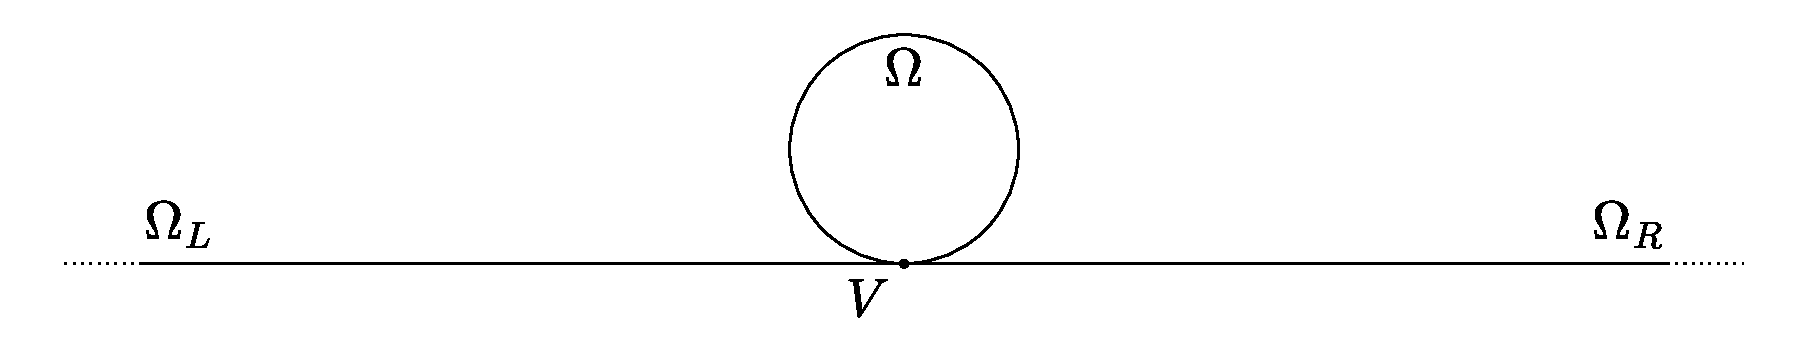
\includegraphics[width=\textwidth,keepaspectratio]{graph.eps}
\caption{квантовый граф $\Gamma$, состоящий из полубесконечных ребер $\Omega_L, \Omega_R$ и рассеивателя $\Omega$, представляющего из себя окружность длиной $1$.}
\end{figure}

Мы рассматриваем случай рассеяния волны c волновым вектором $k$, приходящей слева направо. Таким образом, волновые функции на различных частях графа принимают следующий вид:

\begin{align*}
\psi_L(x) &= \eexp{\iu k x} + R \eexp{-\iu k x} \\
\psi_R(x) &= T \eexp{\iu k x}\\
\psi_\Omega(x) &= P \sin(k x) + Q \cos(k x)
\end{align*}
, где $R$ и $T$ — коэффициенты отражения и прохождения волны. Так как система симметрична, ее матрица рассеяния принимает вид
$S(k) = \begin{pmatrix} R(k) & T(k) \\ T(k) & R(k) \end{pmatrix}$.

В вершине $V$ мы ставим граничное условие Дирихле на волновую функцию, и условие $\delta$-барьера высотой $a$ на ее производную:

\begin{align*}
\psi_L(0) = \psi_R(0) = \psi_\Omega(0) = \psi_\Omega(1) \\ 
-\psi'_L(0) + \psi'_\Omega(0) - \psi'_\Omega(1) + \psi'_R(0) = a \psi_L(0)
\end{align*}


\section{Вычисление S-матрицы}
Определим коэффициенты прохождения и отражения, решив систему линейных уравнений:
\begin{align*}
& 1 + R &= T \\
& 1 + R &= Q \\
& Q \cos k + P \sin k &= T \\
& -P k \cos k + Q k \sin k + P k + \iu R k + \iu T k - \iu k &= T a
\end{align*}

Решив систему, получаем:

\begin{align*}
R(k) = -\frac{2 \, k \cos\left(k\right) + a \sin\left(k\right) - 2 \, k}{2 \, k \cos\left(k\right) + {\left(a - 2 i \, k\right)} \sin\left(k\right) - 2 \, k} \\
T(k) = -\frac{2 i \, k \sin\left(k\right)}{2 \, k \cos\left(k\right) + {\left(a - 2 i \, k\right)} \sin\left(k\right) - 2 \, k}
\end{align*}
, подставляя полученные значения коэффициента прохождения и отражения в S-матрицу, получаем:
\[
\det S = 
\frac
{\cos\left(k\right) + {\left(\frac{a}{2 k} + i\right)} \sin\left(k\right) - 1}
{\cos\left(k\right) + {\left(\frac{a}{2 k} - i\right)} \sin\left(k\right) - 1}
\]


\section{Исследование полноты при $a=0$}
Рассмотрим случай $a=0$:
\[
\det S
= \frac
{\cos\left(k\right) + \iu \sin\left(k\right) - 1}
{\cos\left(k\right) - \iu \sin\left(k\right) - 1}
= \frac{\eexp{\iu k} - 1}{\eexp{-\iu k} - 1}
= -\eexp{i k}
\]

\[
\ln \abs{\det S} = \ln \eexp{- \Im k} = -\Im k
\]

% Преобразование Кэли: $\zeta = \frac{k - i}{k + i}$, обратное: $k = \iu \frac{1 + \zeta}{1 - \zeta}$.

Вычислим интеграл в пространстве единичного диска, для этого применим обратное преобразование Кэли $k \to \iu \frac{1 + \zeta}{1 - \zeta}$, отображающее $\{ z \vert \Im z \ge 0 \}$ в $\bbD$, к подынтегральной функции: $\Im k \to \Im \left( \iu \frac{1 + \zeta}{1 - \zeta} \right) $.

\[
  \lim\limits_{R = 1} \int\limits_{\abs{\zeta} = R} \ln \abs{\det S(\zeta)} d \zeta
= \lim\limits_{R = 1} \int\limits_{\abs{\zeta} = R} \Im \left( \iu \frac{1 + \zeta}{1 - \zeta} \right)  d\zeta = \dots
\]

Перейдем в полярные координаты: $\zeta \to R \eexp{\iu \phi}, d\zeta \to R \iu \eexp{\iu \phi}$:
\[
\dots = \lim\limits_{R = 1} \int\limits_{\abs{\zeta} = R} \Im \left( \iu \frac{1 + R \eexp{\iu \phi}}{1 - R \eexp{\iu \phi}} \right) R \iu \eexp{\iu \phi} d\phi
\]

Комплексный интеграл складывается из сумм интегралов действительной и мнимной части подынтегрального выражения. Рассчитаем мнимую часть:

\begin{align*}
\Im \left(  \Im \left( \iu \frac{1 + R \eexp{\iu \phi}}{1 - R \eexp{\iu \phi}} \right) R \iu \eexp{\iu \phi} \right)
 &= R \Re \left(  \Re \left( \frac{1 + R \eexp{\iu \phi}}{1 - R \eexp{\iu \phi}} \right) \eexp{\iu \phi} \right) \\
 &= R \Re \left( \frac{1 + R \eexp{\iu \phi}}{1 - R \eexp{\iu \phi}} \right) \Re \left(   \eexp{\iu \phi} \right) \\
 &= R \Re \left( \frac{(1 + R \eexp{\iu \phi}) (1 - R \eexp{-\iu \phi}) }{(1 - R \eexp{\iu \phi}) (1 - R \eexp{-\iu \phi})} \right) \cos \phi \\
 &= R \Re \left( \frac{1 - R^2 + 2 \iu R \sin \phi}{1 + R^2 - 2 R \cos \phi} \right) \cos \phi \\
 &= R \frac{1 - R^2}{1 + R^2 - 2 R \cos \phi} \cos \phi \\
 % NOTE calculate the integral properly?
 &= 2 \pi R^2
\end{align*}

Можно видеть, что предел мнимой части при $R \to 1$ равен $2 \pi$, следовательно, по критерию полноты, система резонатных состояний графа $\Gamma$ не является полной на кольце $\Omega$.


\section{Заключение}
В работе была строго аналитически показана неполнота резонансных состояний на резонаторе типа кольца. Данное исследование является важной подзадачей в более общей задаче нахождения пространства, в котором резонансные состояния квантового графа будут образовывать полную систему, так как в произвольном квантовом графе ребра могут соединять либо две разные вершины, либо быть петлей (что и является резонатором типа кольца).

Естественным продолжением данной работы может являться исследование полноты системы резонансных состояний при других граничных условиях в точке соединения резонатора и волновода.

% \section*{Благодарности}
% Текст.

\begin{thebibliography}{99}
\bibitem{1} Kuchment P. \textit{Waves in Random Media}, \textbf{12}(4), R1-R24 (2002)

\bibitem{2} Lobanov I.S., TrifanovA.I., Trifanova E.S. \textit{Nanosystems: Phys. Chem. Math.}, \textbf{3}(4), 512-523 (2013).

\bibitem{3} Exner P., Keating J.P., Kuchment P., Sunada T., Teplyaev A., (eds.) \textit{Analysis on Graphs and Its Applications}. Proc. Symp. Pure Math., 77 (Providence, RI: Amer. Math. Soc.) (2008)

\bibitem{4} Popov I.Yu., Skorydina A.N., Blinova I.V. \textit{J. Math. Phys.}, \textbf{55}, 033504 (2014)

\bibitem{popov_exner70} Popov I.Yu., Popov A.I. {\it 1D model of the Helmholtz resonator}. Manuscript (2016)

\bibitem{nikolskii} Nikol'skii N.K. {\it Treatise on the Shift Operator: Spectral Function Theory}.  Springer Berlin Heidelberg,  491~p. (2012)

\end{thebibliography}

\end{document}
